\chapter{O InvestMVC}

\section{Arquitetura Orientada a Componentes}

Arquitetura Orientada a Componentes possui o propósito de dividir para conquistar. Um grande problema é quebrado em partes menores e em seguida se desenvolve soluções mais elaboradas \cite{john}.

Por usar vários paradigmas, a ferramenta InvestMVC terá vários componentes e cada componente terá seu paradigma de programação e responsabilidade bem definida, como mostrado na Figura \ref{componente}.

\begin{figure}[H]
\centering
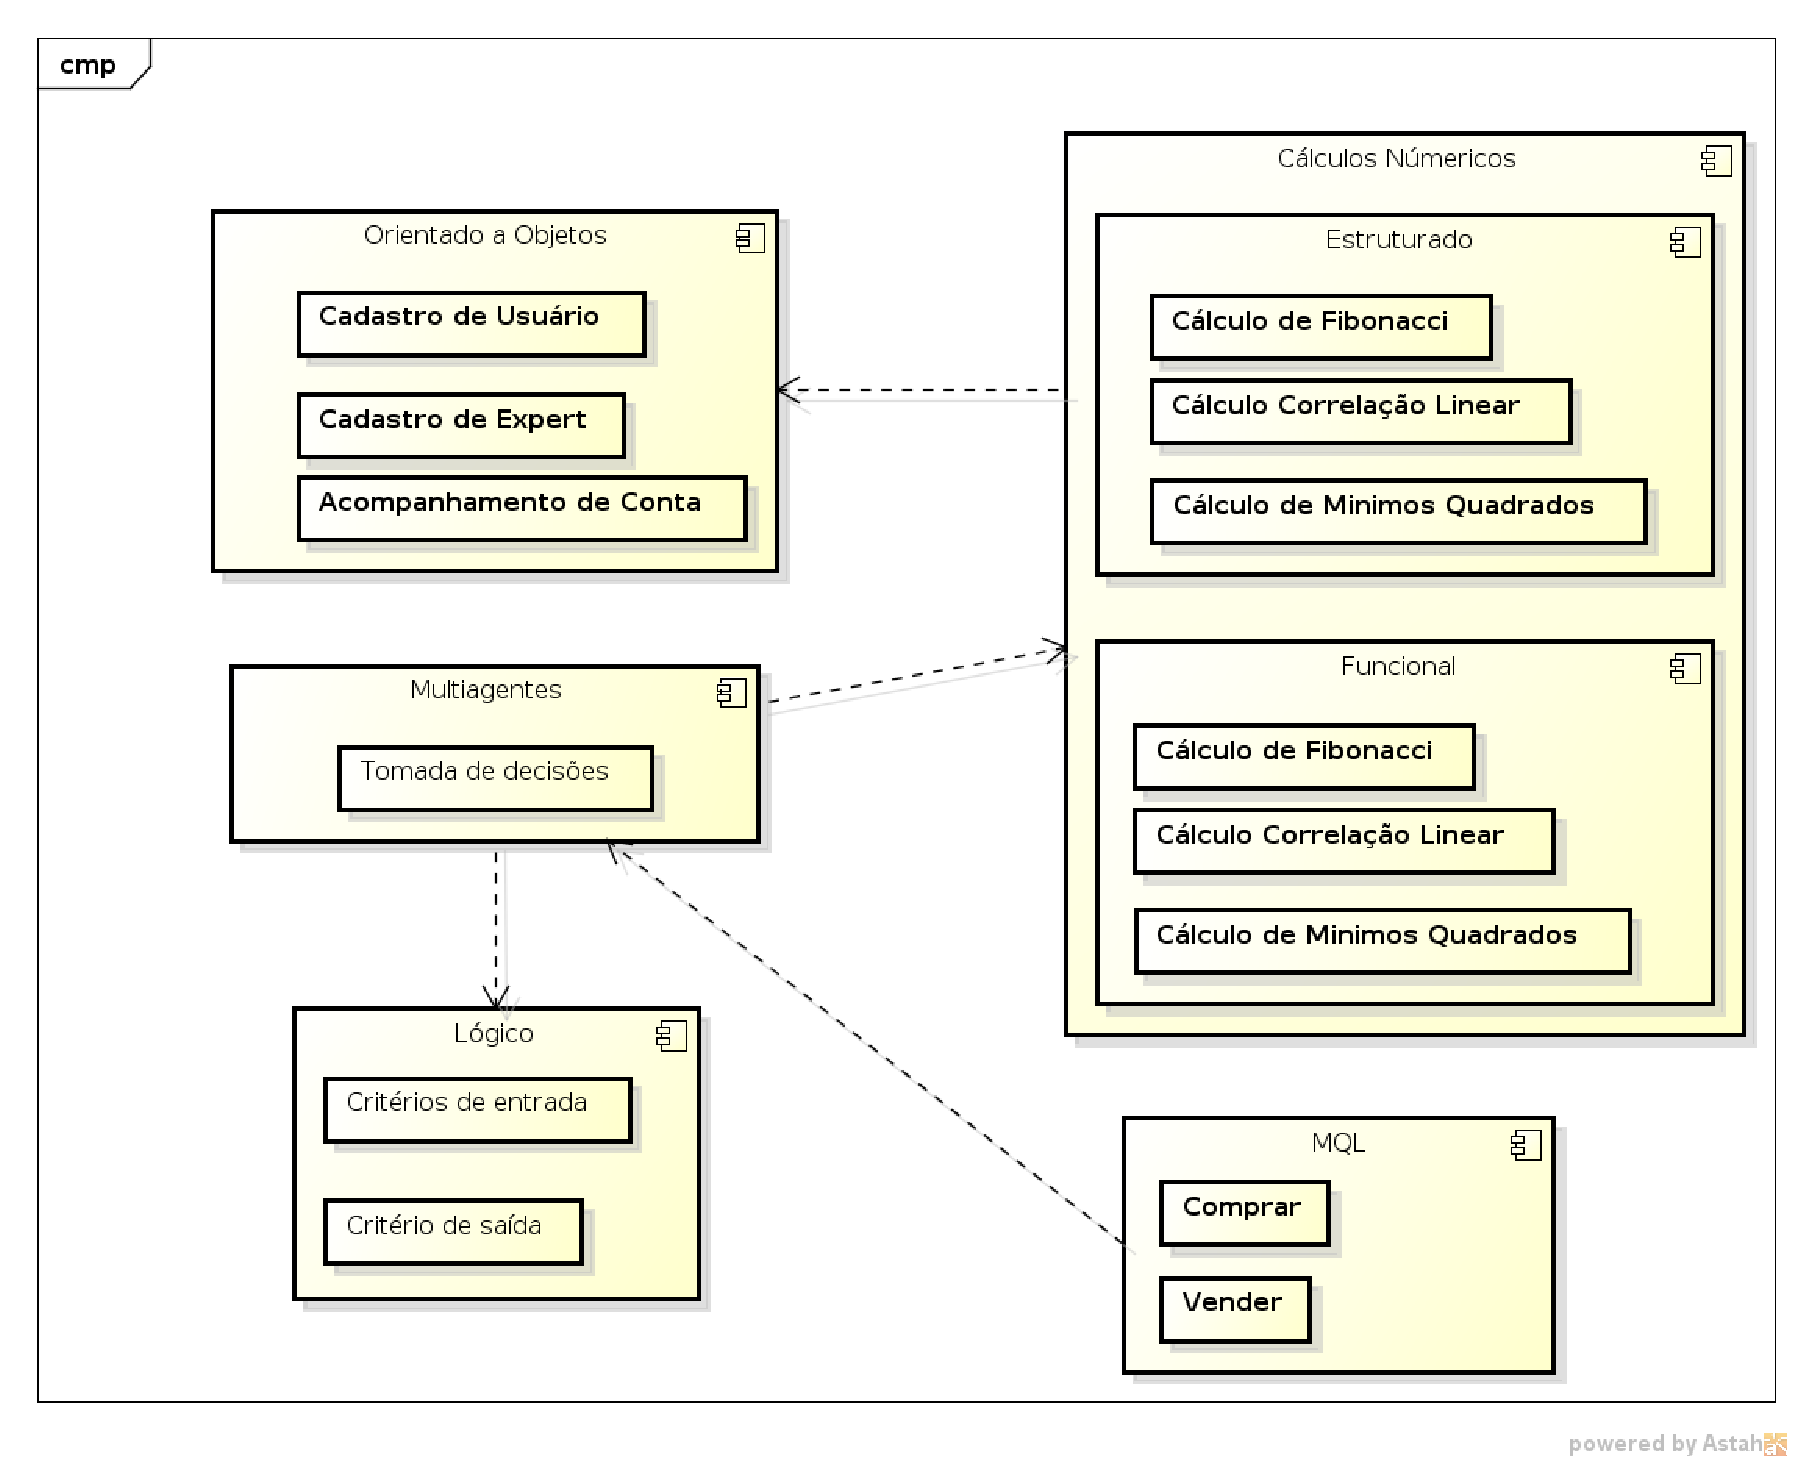
\includegraphics[width=0.9\textwidth]{figuras/componente}
\caption{Diagrama de Sequência InvestMVC}
\label{componente}
\end{figure}

\subsection{Componente Orientado a Objetos}

Este componente fará a interação com o usuário e será implementado em linguagem Grovvy. A escolha dessa linguagem, se deu porque esta é voltada para aplicações web e juntamente com  o framework grails, fornece a criação de um projeto com uma arquitetura MVC definida, como demonstra a Figura \ref{classeOO}.

\begin{figure}[H]
\centering
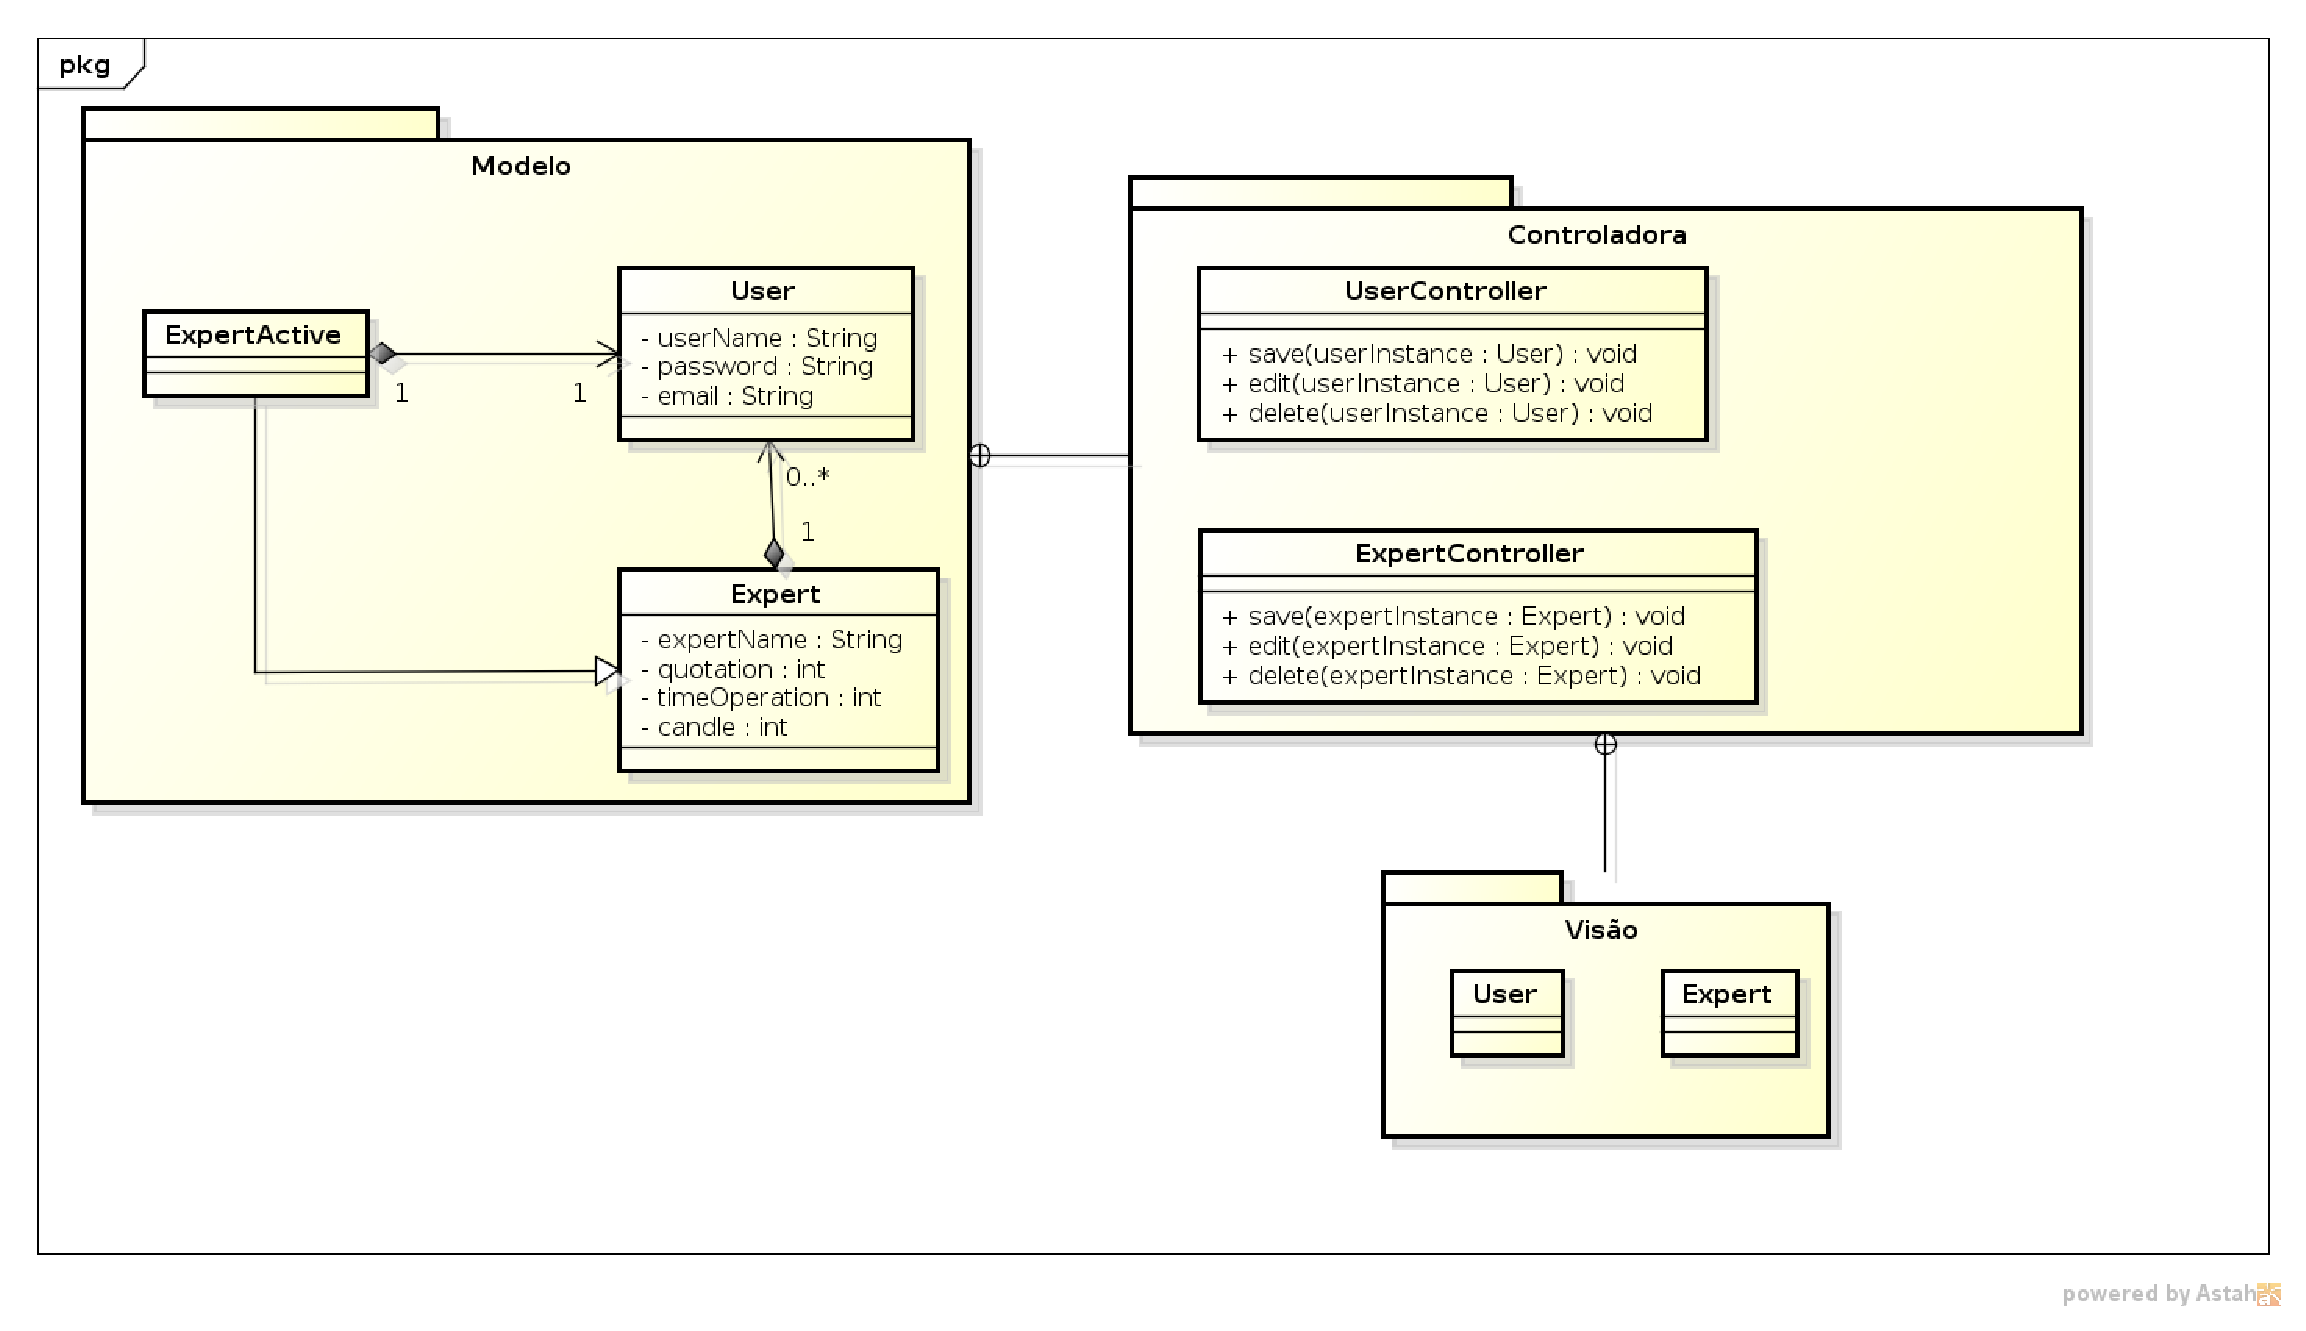
\includegraphics[width=0.9\textwidth]{figuras/classeOO}
\caption{Diagrama de Classe InvestMVC componente Orientado a Objetos} 
\label{classeOO}
\end{figure}

Segundo \citeonline{lamin} na arquitetura MVC o controle de fluxo de dados dentro deste módulo ocorre da seguinte forma:

\begin{enumerate}
\item O usuário,neste caso o investidor, interage com a Visão.
\item A Controladora manipula o evento da interface do usuário através de uma rotina.
\item A Controladora acessa o Model, atualizando-o baseado na interação do usuário.
\end{enumerate}

O diagrama de sequência do componente Orientado a Objetos é evidenciado na Figura \ref{sequenciaOO}.

\begin{figure}[H]
\centering
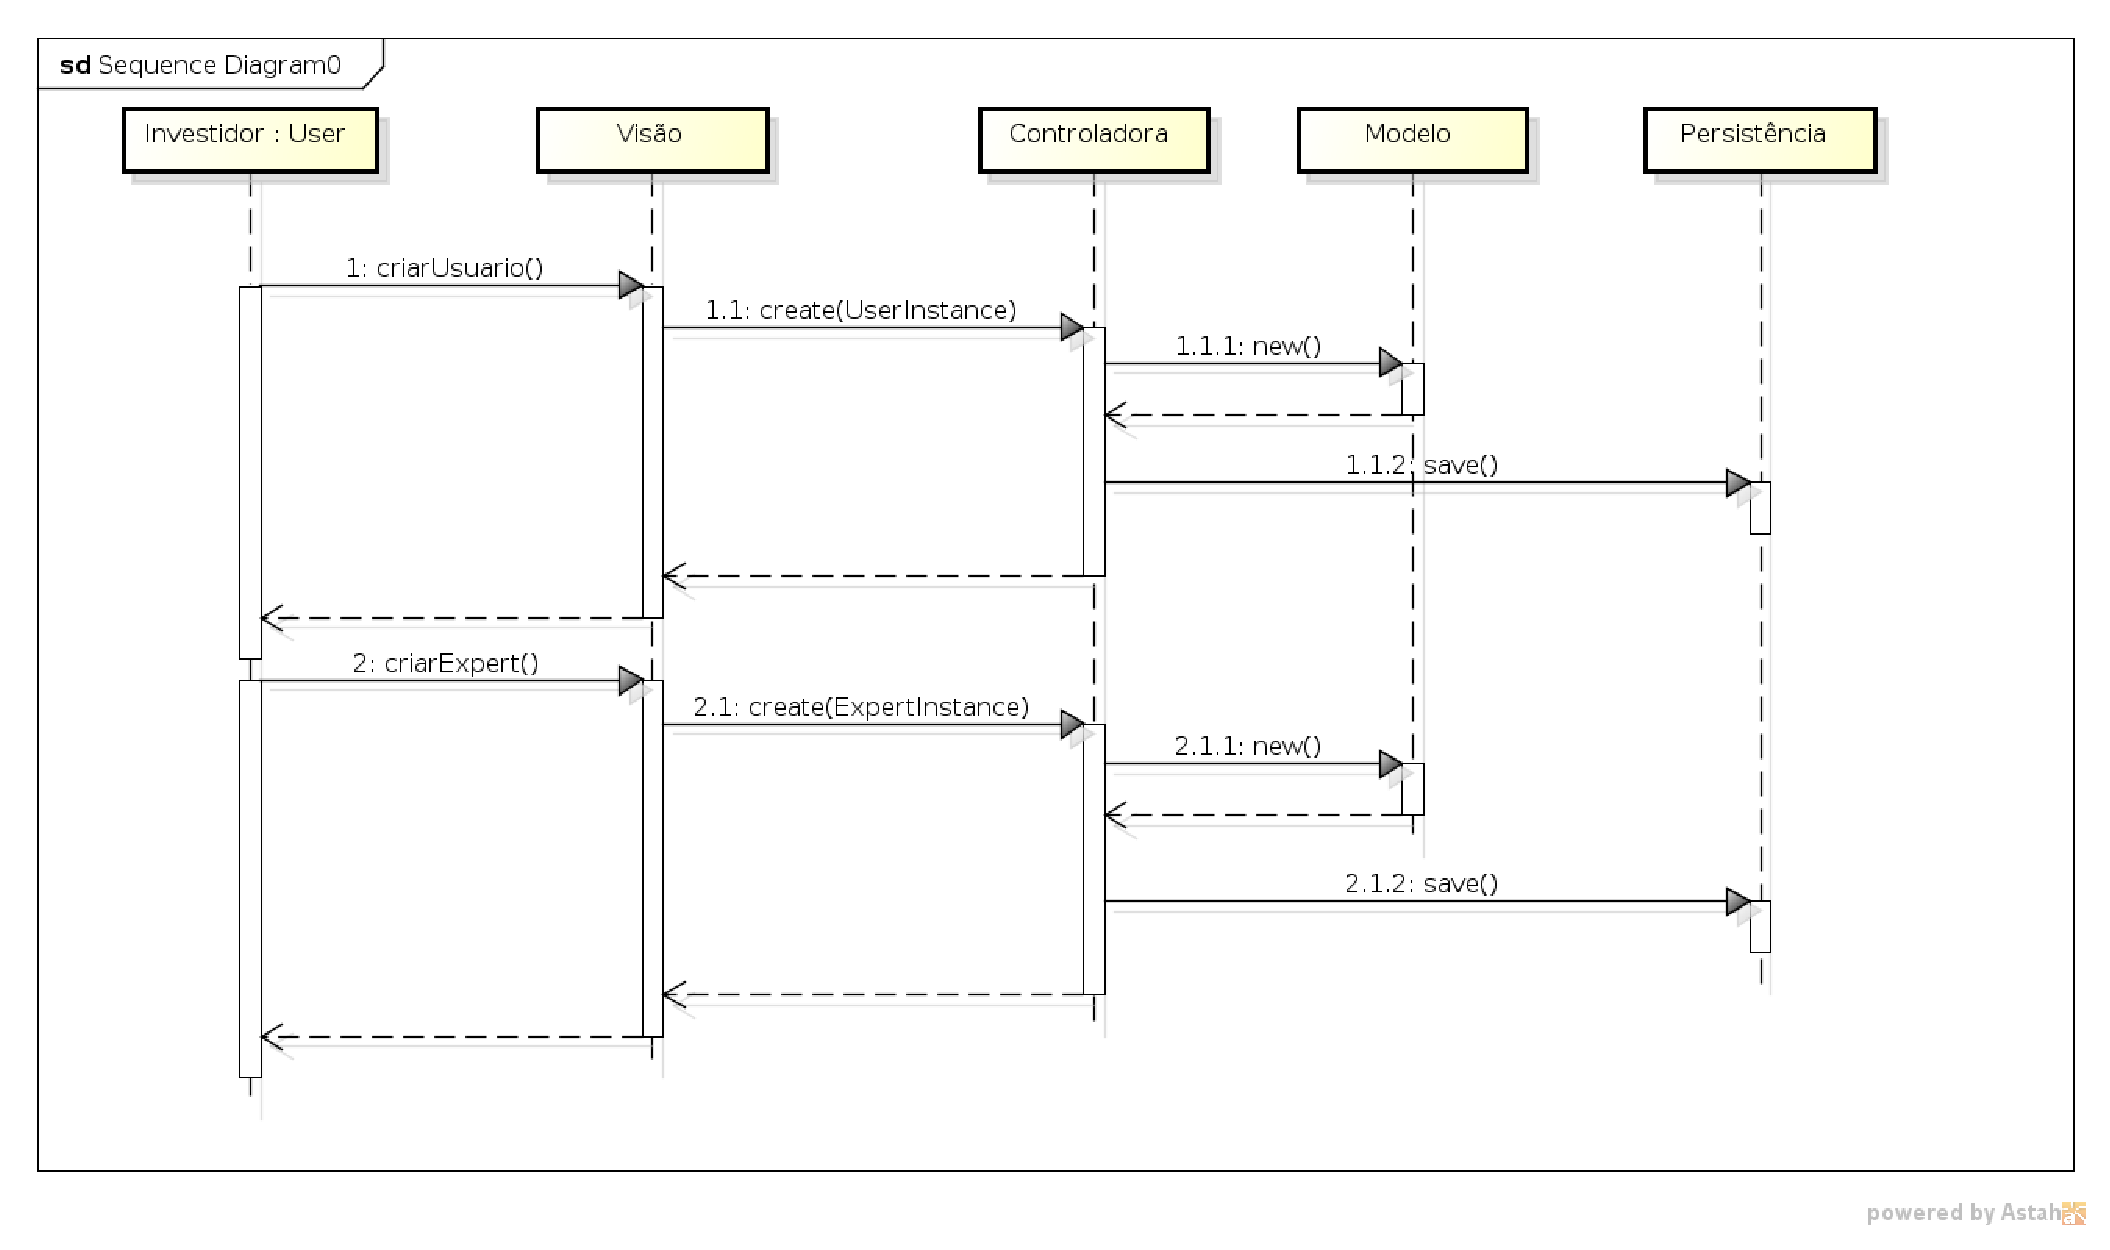
\includegraphics[width=0.9\textwidth]{figuras/sequenciaOO}
\caption{Diagrama de sequência InvestMVC componente Orientado a Objetos}
\label{sequenciaOO}
\end{figure}

\subsection{Componente Cálculos Numéricos}

O componente Cálculos Numéricos será responsável por calcular os Métodos Matemáticos presentes na ferramenta InvestMVC. Este módulo é composto por dois outros módulos: módulo Estruturado e módulo Funcional.

O componente Estruturado da ferramenta InvestMVC será programado em linguagem C e o módulo Funcional em linguagem Haskell. Ambos os componentes irão realizar os mesmos cálculos. Isso aumenta a probabilidade de não ocorrer erros nos cálculos dos Métodos Matemáticos. Caso um dos componentes por algum motivo não seja executado no momento correto, a tendência é que o outro módulo realize os cálculos.

\subsubsection{Componente Funcional}
Por ser uma linguagem de programação funcional sua "gramática" está próxima das funções matemáticas, logo a implementação dos métodos algébricos e numéricos se torna muito intuitiva. \cite{hoogle2013}.

O paradigma funcional é declarativo, por limitar o uso de atribuições à variáveis suas funções são mais precisas do que em outros paradigmas \cite{piponi2006}.

Devido aos fatos externalizados, o paradigma funcional, foi eleito para implementar os Métodos Matemáticos de Correlação Linear, Mínimos Quadrados e Fibonacci. Por ser simples,este componente será formado apenas por seus 4 arquivos haskell, cada arquivo realiza o cálculo de um Método Numérico, com execeção do arquivo  Arquivos.hs, que faz a leitura de arquivos.

\begin{figure}[H]
\centering
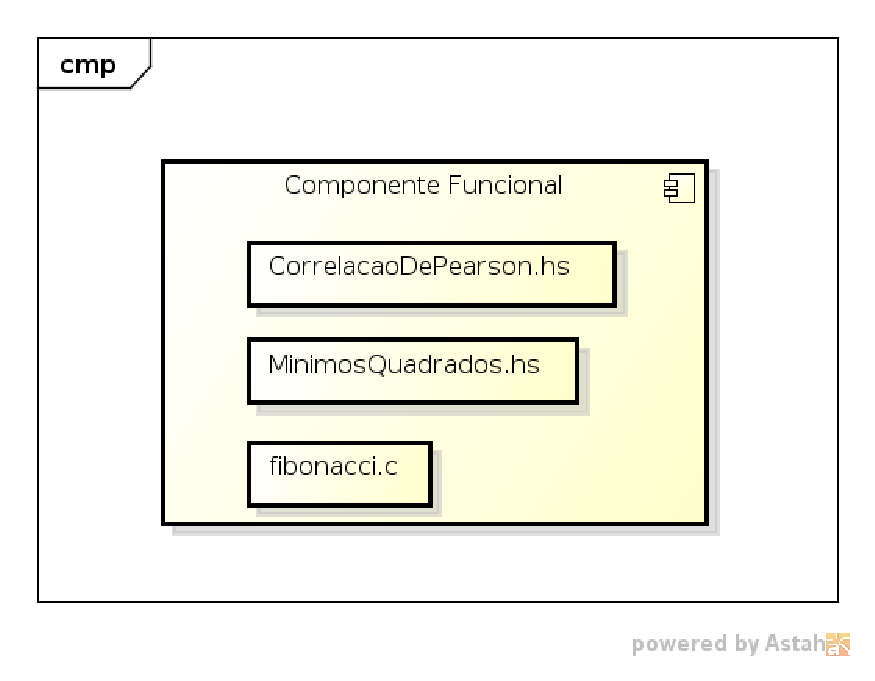
\includegraphics[width=0.5\textwidth]{figuras/componenteFuncional}
\caption{Componente Funcional InvestMVC} 
\label{componenteFuncional}
\end{figure}

O componente Funcional espera uma socilitação de cálculo do componente Multiagente, logo após a solicitação o componente busca na persistência(um arquivo) as cotações do mercado, com estas cotações o componente é capaz de realizar o cálculo do Método Numérico que é esperado pelo componente Multiagente, como é mostrado na Figura \ref{sequenciaFuncional}.

\begin{figure}[H]
\centering
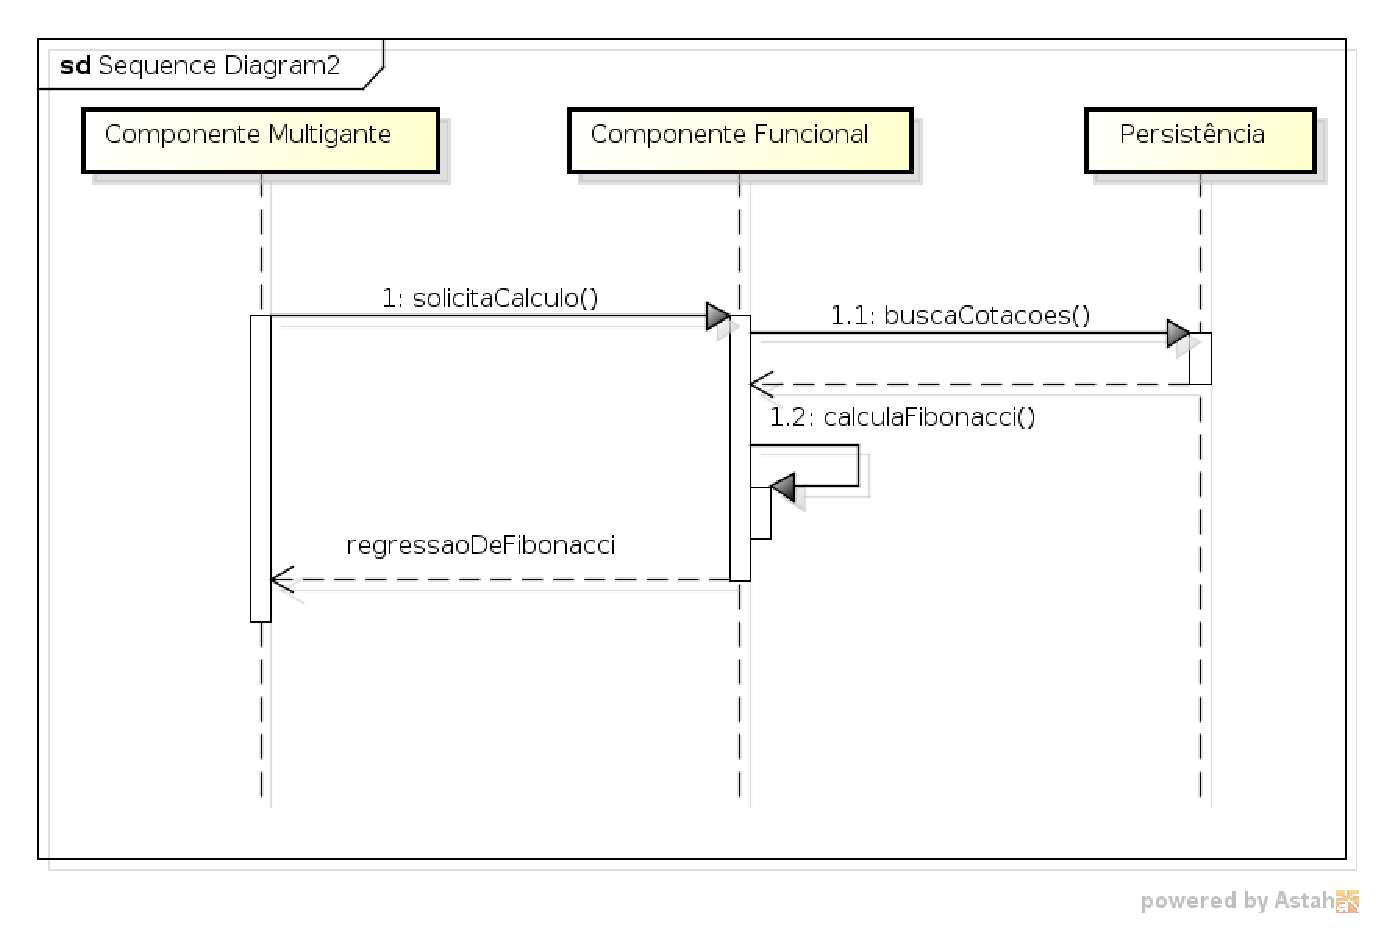
\includegraphics[width=0.9\textwidth]{figuras/sequenciaFuncional}
\caption{Diagrama de Sequência do Componente Funcional InvestMVC} 
\label{sequenciaFuncional}
\end{figure}

\subsubsection{Componente Estruturado}

A linguagem de programação C é estruturada e possui a vantagem da velocidade de execução do código fonte. Também é uma linguagem bastante utilizada para realizar cálculos numéricos e algébricos \cite{gustavo}. 

Devido aos fatos externalizados, o paradigma estruturado utilizando a linguagem C, também foi eleito para implementar os Métodos Matemáticos de Correlação Linear, Mínimos Quadrados e Fibonacci.

A arquitetura e sequência do fluxo de dados do Componente Estruturado segue a mesma lógica do Componente Funcional, como ilustrado na Figura \ref{sequenciaEstruturado}.

\begin{figure}[H]
\centering
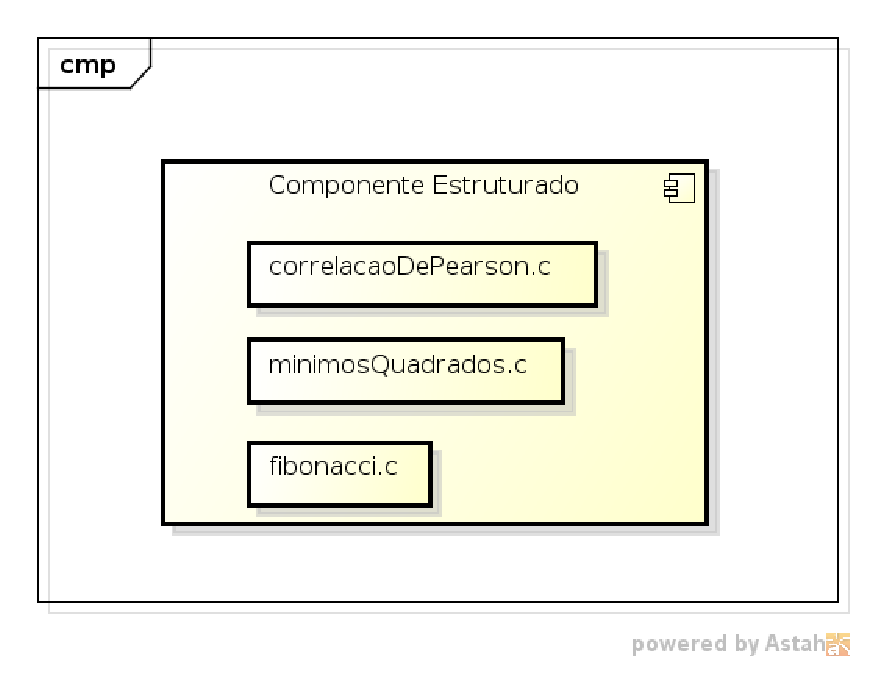
\includegraphics[width=0.7\textwidth]{figuras/componenteEstruturado}
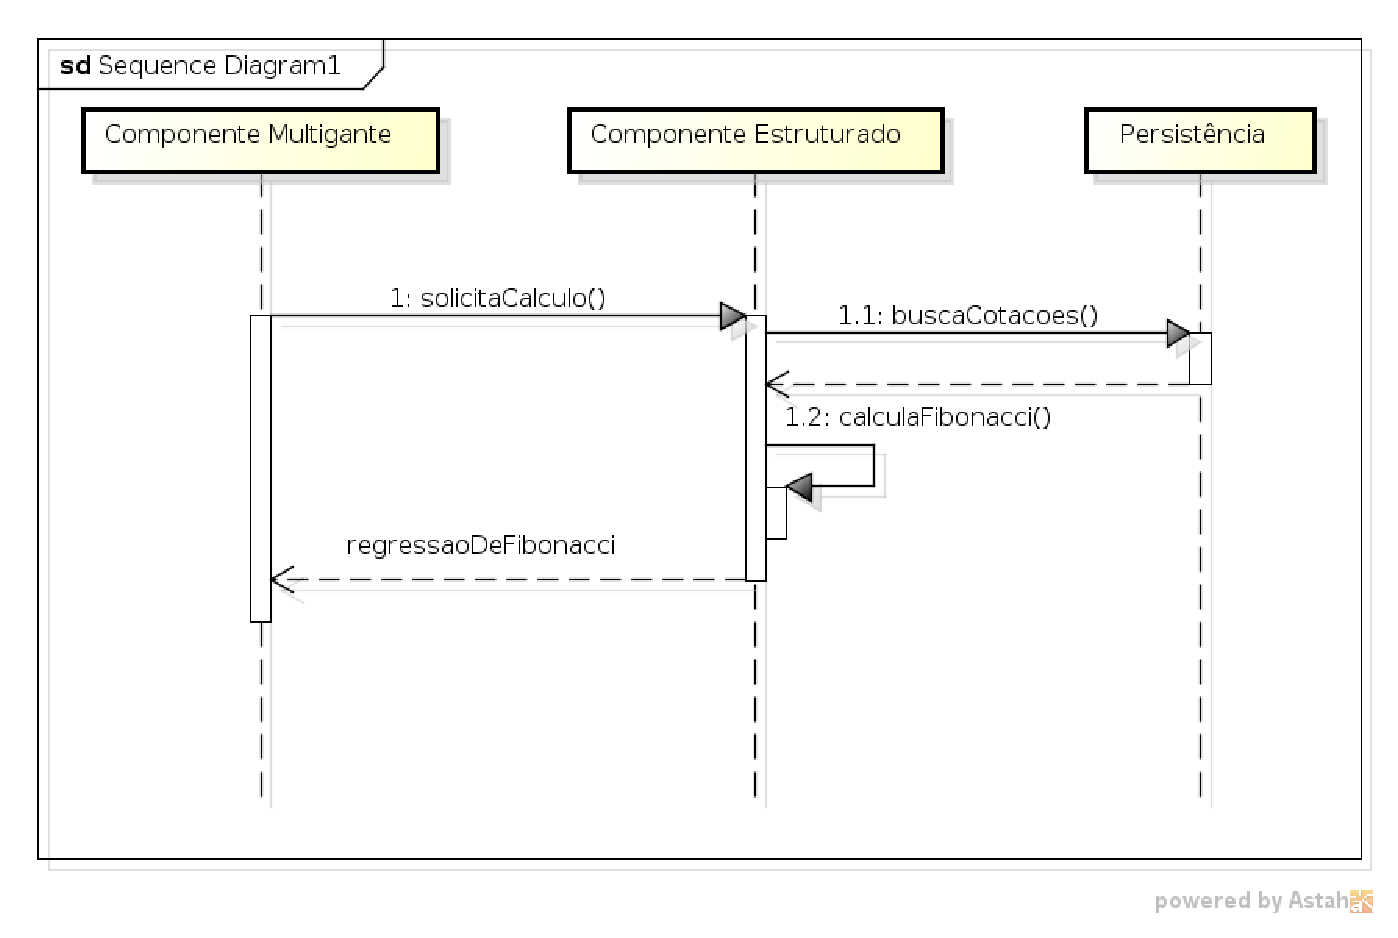
\includegraphics[width=0.7\textwidth]{figuras/sequenciaEstruturado}
\caption{Diagramas de Componentes e de Sequência do Componente Estruturado InvestMVC.}
\label{sequenciaEstruturado}
\end{figure}

\subsection{Componente Multiagentes}

O componente Multiagente será implementado usando o paradigma Multiagente com linguagem Java. 

Agentes de software são entidades autônomas e com capacidades sociais, o uso deste paradigma justifica-se na tomada de decisões \cite{agentBuilderWhy}. 

Os agentes da ferramenta  InvestMVC possuem uma arquitetura reativa, pois suas ações se dão pelas variações que ocorrem nas cotações do Mercado de Moedas.

A arquitetura do Componente Multiagente está modularizado por pacotes: o pacote comportamentos será formado por compormentos que serão usados pelos Agentes de Software, o pacote metodosNumericos será formado por Agentes que acerão o componente Cálculos Numéricos, o pacote investidores será composto por Agentes que vão interagir com o Componente MQL e o pacote execucao iniciará a execução do SMA.

\begin{figure}[H]
\centering
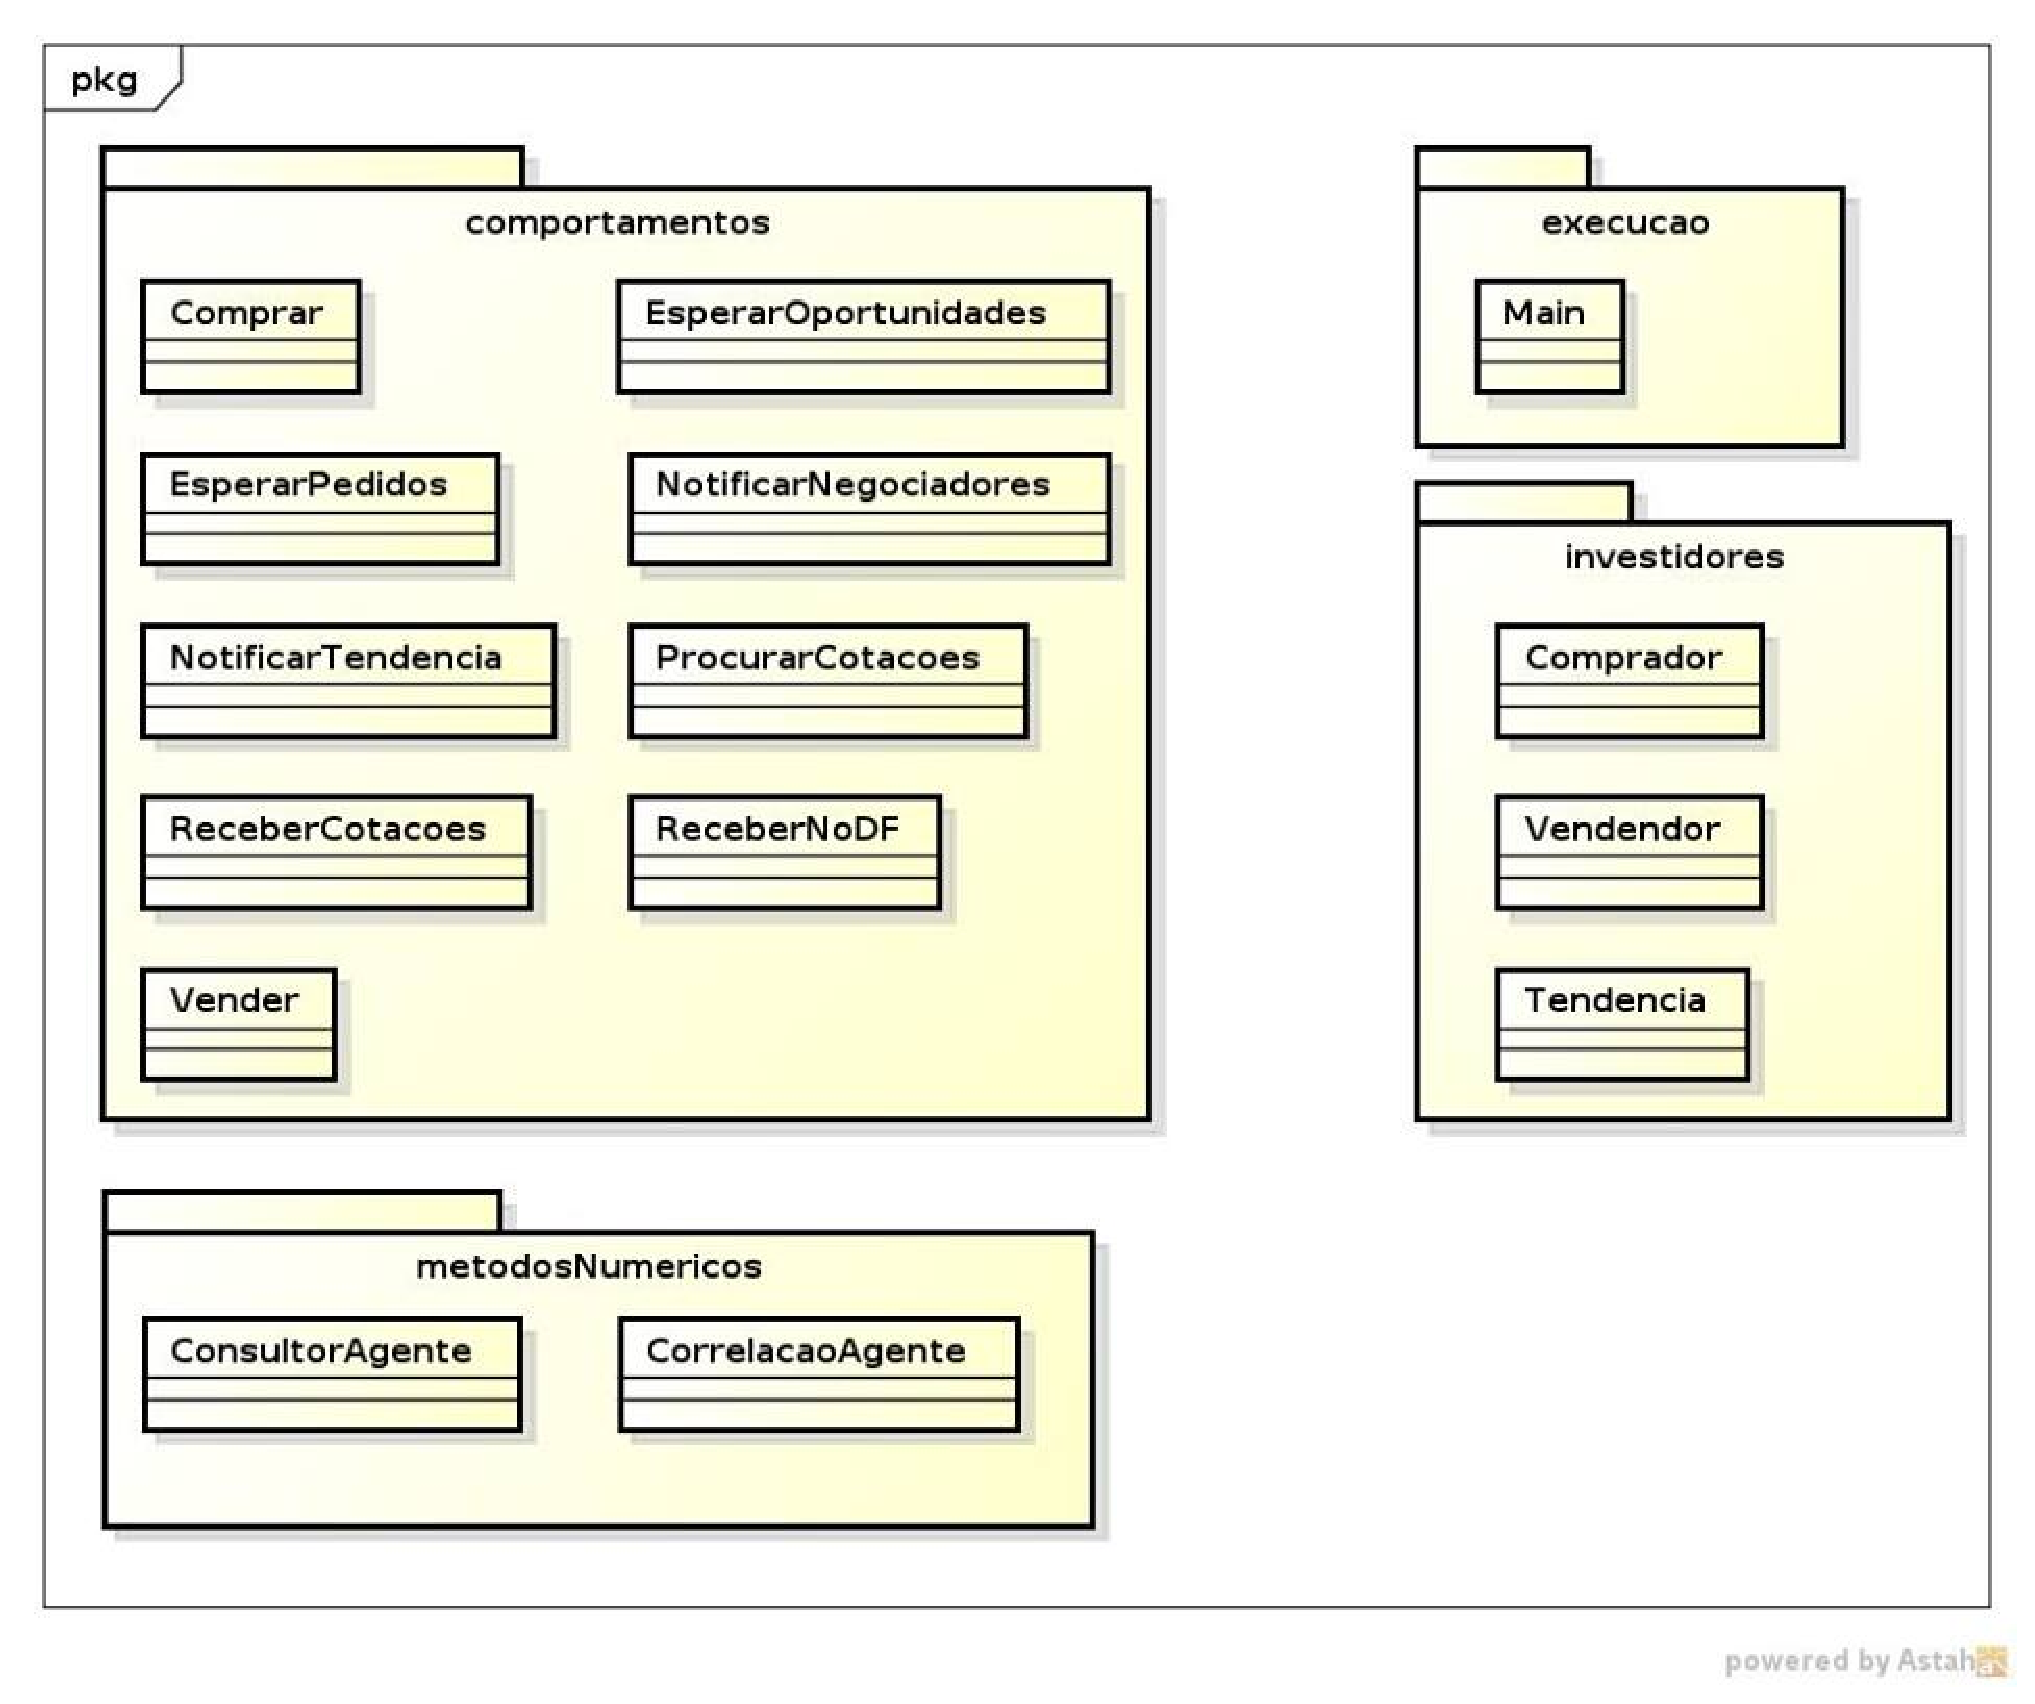
\includegraphics[width=0.9\textwidth]{figuras/diagramaClassesSMA}
\caption{Diagrama de Classe do Componente Multiagente InvestMVC} 
\label{diagramaClassesSMA}
\end{figure}

\subsection{Componente Lógico}

O componente Lógico será produzido em linguagem Prolog e vai definir uma base de conhecimento que servirá como critério de entrada e saída no Mercado de Moedas.

O paradigma Lógico facilita a representação, inserção e recuperação de conhecimento, por isso é muito usado em aplicações com Inteligência Artificial \cite{almeida2010}.

A interação do Componente Lógico com o Componente Multiagentes é evidenciada na Figura \ref{sequenciaLogico}.

\begin{figure}[H]
\centering
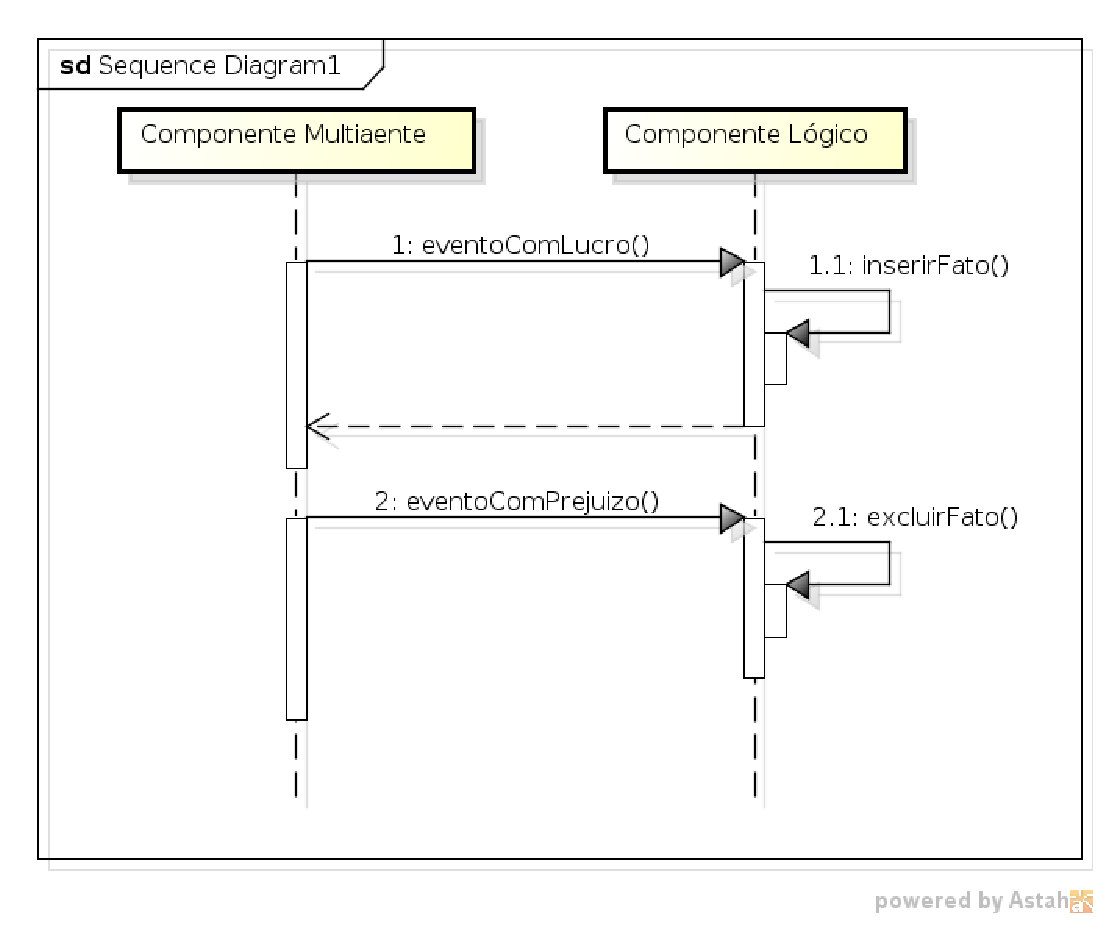
\includegraphics[width=0.7\textwidth]{figuras/sequenciaLogico}
\caption{Diagrama de Sequência do Componente Lógico InvestMVC.}
\label{sequenciaLogico}
\end{figure}

\subsection{Componente MQL}

O componente MQL será responsável por receber a resposta do Componente Multiagentes para realizar uma compra ou venda. Também será recebido outros atributos relacionados a compra ou venda, como alavancagem, stop loss e take profit.

A interação do Componente MQL com o Componente Multiagentes é evidenciada na Figura \ref{sequenciaMQL}.

\begin{figure}[H]
\centering
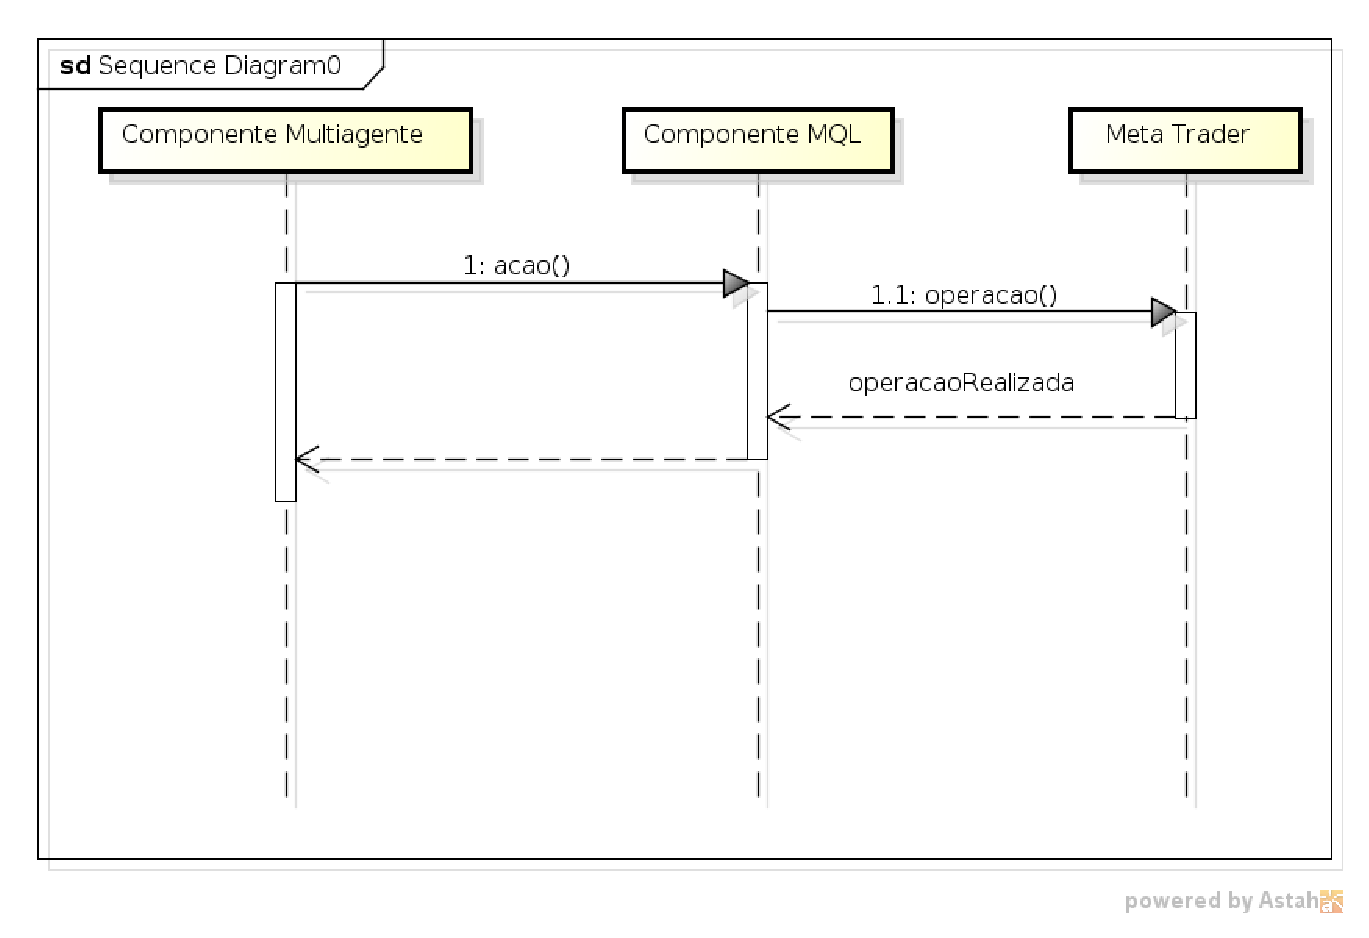
\includegraphics[width=0.5\textwidth]{figuras/sequenciaMQL}
\caption{Diagrama de Sequência do Componente MQL InvestMVC.}
\label{sequenciaMQL}
\end{figure}

\subsection{Fluxo de atividades  da ferramenta InvestMVC}

O investidor interage apenas com o componente Orientado a Objetos, criando seu usuário e Experts, no qual serão persistidos. Além disso, o investidor também poderá ativar um Expert.

O componente Multiagentes vai verificar a tendência do Mercado de Moedas, por meio da plataforma MetaTrader. Sendo assim, o componente Multiagentes buscará na persistência o Expert que está ativo. Sabendo qual o Expert que foi ativado, o componente Multiagente faz a requisição de cálculos para os módulos C e Haskell. A partir desse resultado, o componente Multiagente procurará no Módulo Base de Conhecimento, a alavancagem (quanto deve arriscar) e os valores de entrada para o método de Correlação de Pearson, Fibonacci e Mínimos Quadrados. Caso todas as especificações para o módulo Multiagentes sejam obedecidas, ele informa ao componente MQL para realizar uma compra ou venda.

\begin{figure}[H]
\centering
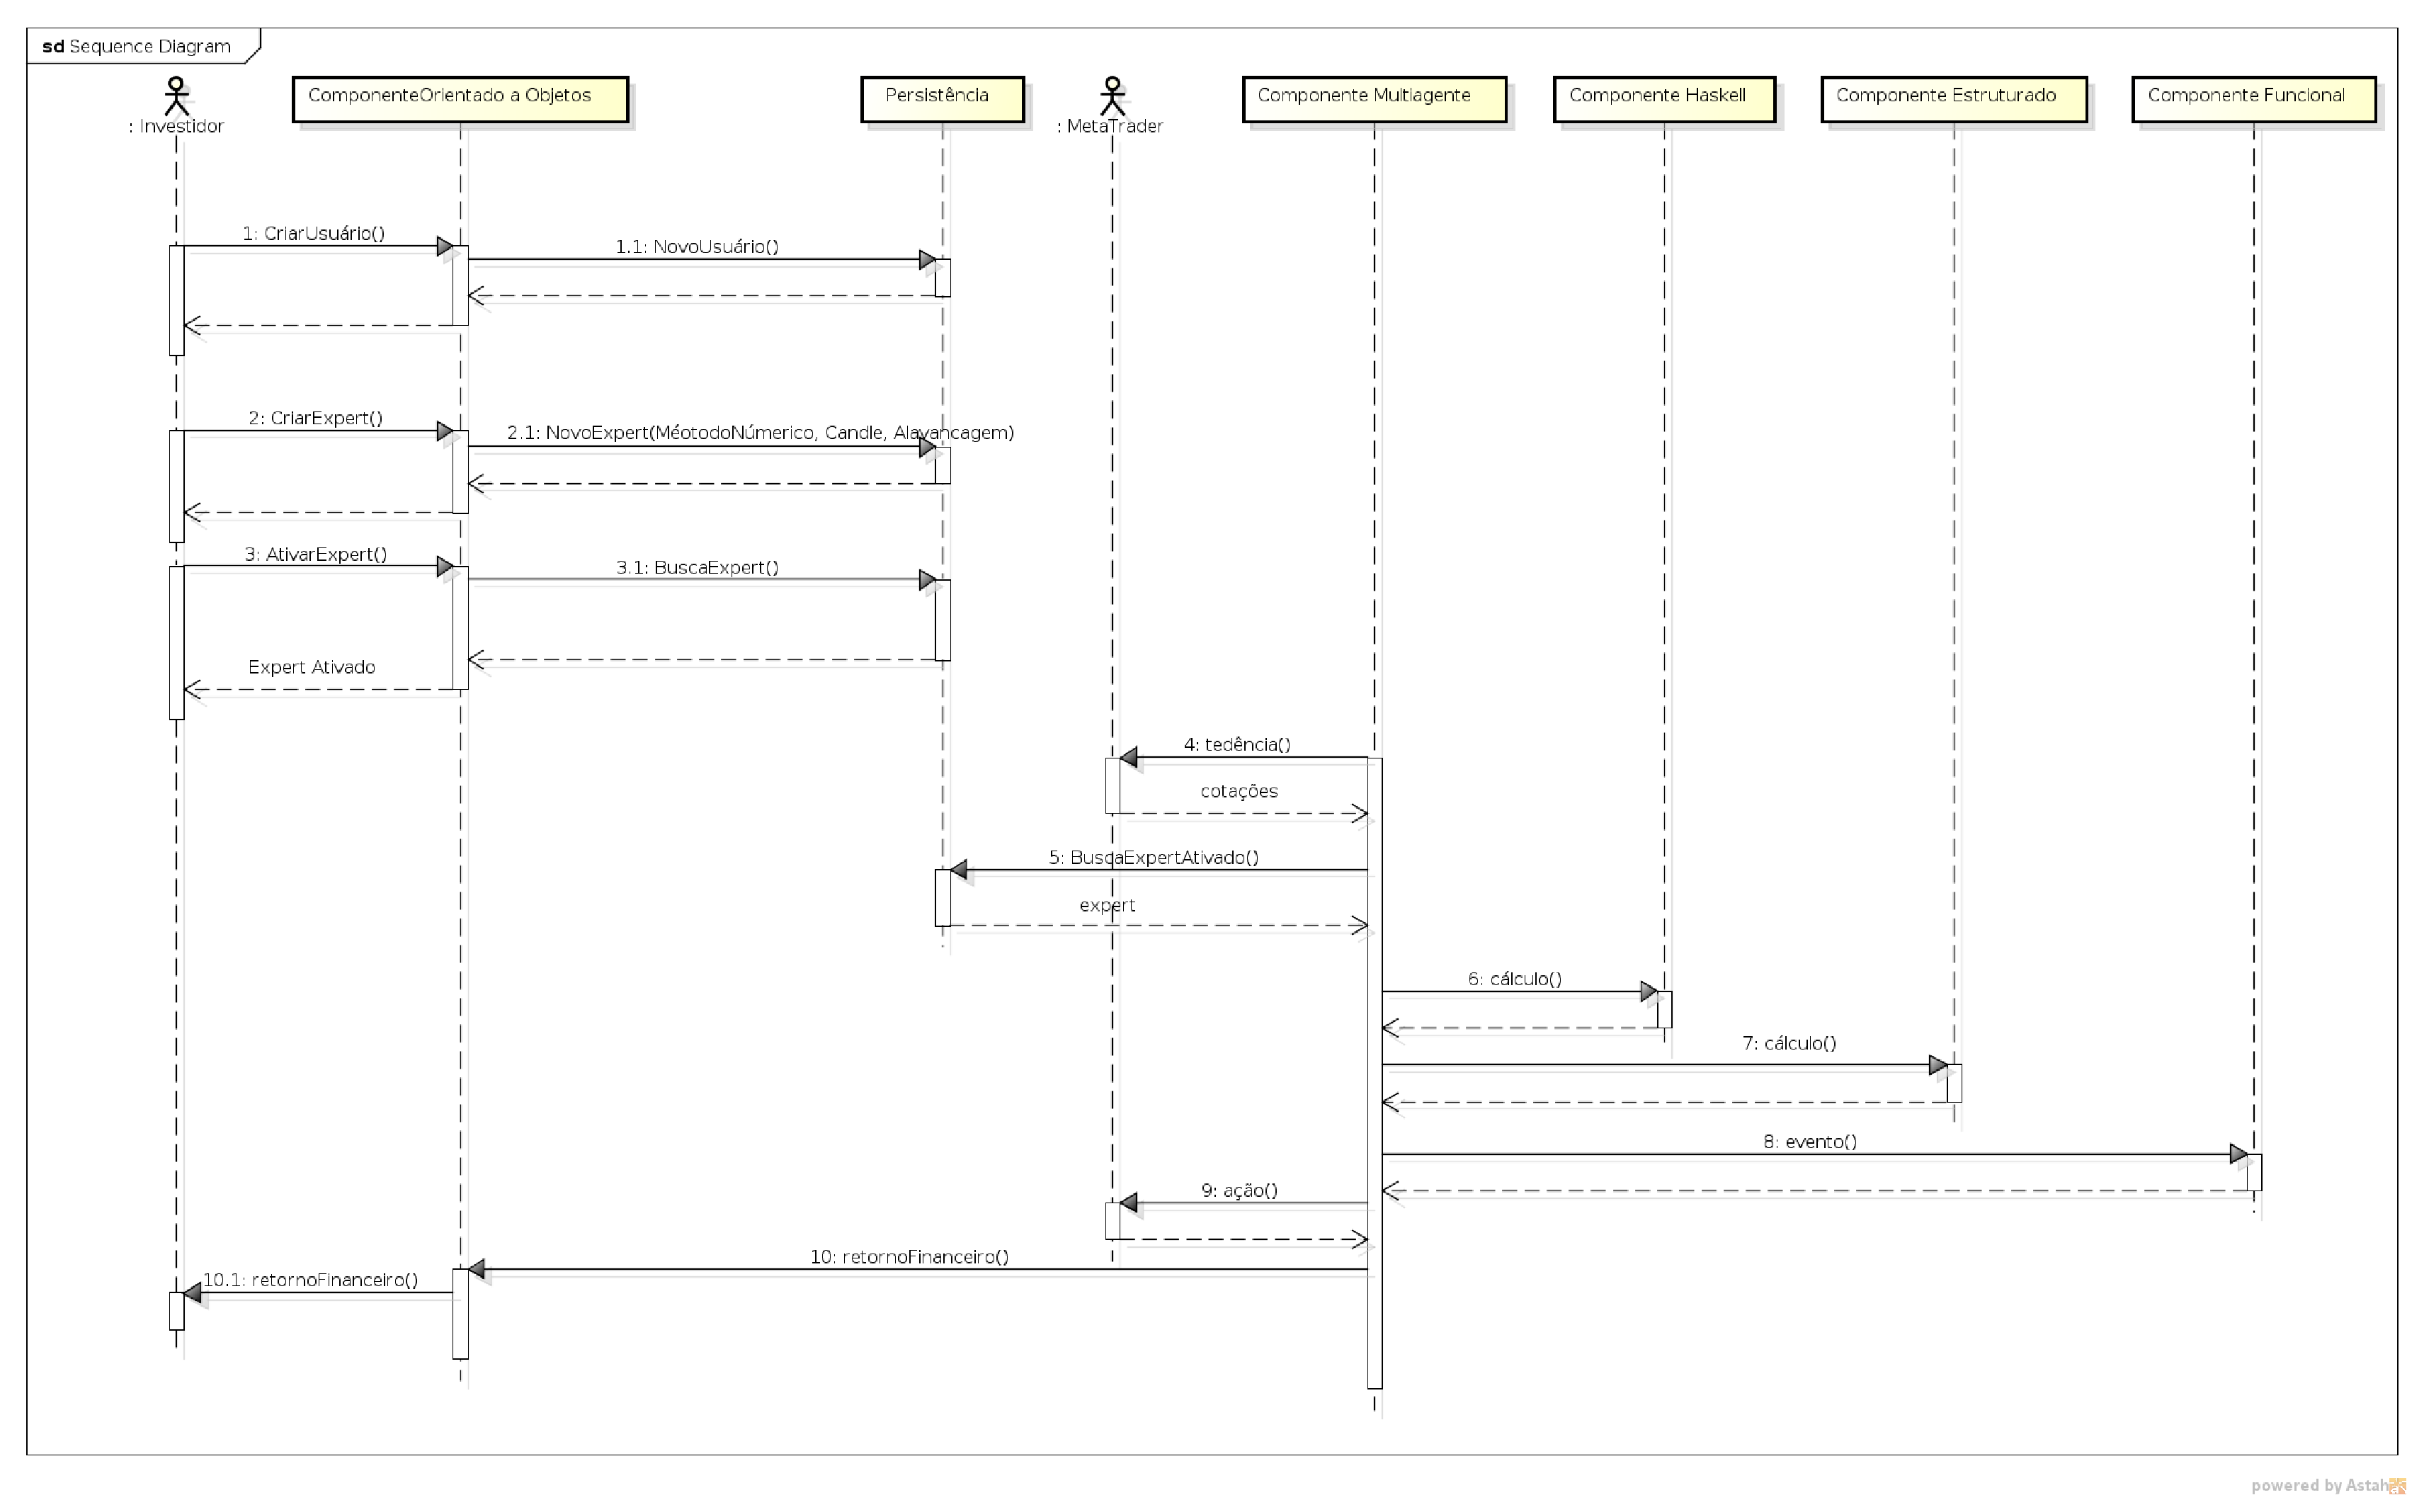
\includegraphics[width=0.9\textwidth]{figuras/sequencia}
\caption{Diagrama de Sequência InvestMVC} 
\label{sequencia}
\end{figure}
